\documentclass{article}
\usepackage[utf8]{inputenc}

% geometry allows us to change the dimensions of the paper
\usepackage{geometry}
\geometry{
    top = 4cm,
    bottom = 3cm,
    left = 2cm,
    right = 2cm,
    headsep = 2cm
}
\usepackage{graphicx}

% packages that I have imported
\usepackage{hyperref}
\hypersetup{
	colorlinks,
	linkcolor={red!50!black},
	citecolor={violet!50!black},
	urlcolor={blue!50!black}
	}

%% general colors
\usepackage{color}
%% this gives more colors
\usepackage[usenames,dvipsnames]{xcolor}
% commenting mechanism
\newcommand{\miles}[1]{{\color{blue} \sf $\pi$ Miles: [#1]}}
\newcommand{\marchelle}[1]{{\color{purple} \sf $\heartsuit$ Marchelle: [#1]}}

\title{Police Accountability: Quantifying Associations Between Charges and Race/Area In Arrest Data}
% Make the authors and include other information
\author{Marchelle Beougher, Miles Mena}
%\address[label1]{Year of 2023, Colorado Springs, CO }
%\ead{milestmena@lewisu.edu}


\date{July 2022}



\begin{document}





\maketitle

\section{Abstract}



The social injustices that mathematics has created within the context of policing, namely predictive policing, has recently begun to be documented and studied within the literature. At the same time, there has been an effort from mathematicians and data scientists to create methods to examine police misconduct and hold departments accountable. This paper proposes some mathematical and data science techniques that can help quantify the differences in how racial groups and areas categorized by economic level are arrested for certain charges, and aims to increase the standard that we hold our law enforcement agencies to. Specifically, we propose using the Chi Squared Test of Independence and the resulting Pearson Residuals to determine if there is a dependent relationship between race and charge or economic level where the arrest takes place and charge and which combinations of these variables drives dependency. Our proposed method is not intended to improve predictive policing models nor are we providing causative explanations for our results.  




\section{Background}

In June of 2020, a large number of mathematicians signed a letter boycotting any work with police departments. This letter was signed in the wake of a string of citizens being killed by police that sparked unrest and protests across the United States. Some mathematicians have historically worked with the police to create algorithms that predict where crime will occur, but the signed letter expressed that these algorithms can be biased and used to justify racism with mathematics.\cite{website:Letter-AMS} 

Beyond this letter, predictive policing has come under sharp critique from some scholars as many of the assumptions within the predictive policing structure are unjustly associated with race.\cite{dirty-data}\cite{examining-predictive-policing} Predictive policing algorithms intake large amounts of historic crime data and train their algorithm to predict where and when crime will occur. The algorithm identifies where crime is concentrated, termed crime hot spots, and attempts to decrease crime in that area by increasing the presence of police officers. As Lum and Isaac have noted, the training data for such an algorithm is filled with human bias, therefore predictive algorithms would implicitly predict crime hot spots in a familiar fashion. In addition, predictive policing assumes that more police in an area deters crime, however it is possible that "crimes that occur in locations frequented by police are more likely to appear in the database simply because that is where the police are patrolling", creating a positive feedback loop.\cite{predict-serve}. 

Predictive policing is meant to both detect crime and deter it, which can create a paradox. Sending a police officer into a hot spot is intended to both catch crime and deter crime. However, if no crime happens when an officer is in an area it can be viewed that either the officer deterred crime from taking place, or that the algorithm was incorrect. On the other hand, if crime does occur at that location, the algorithm is validated but the officer was unable to prevent crime or deter it.  \cite{predictive-reform}

There have been efforts from non-law enforcement organizations to hold police departments accountable such as the Police Scorecard, which gives police departments a quantitative score calculated by the level of police violence, racial bias,and accountability among other factors. This score card provides communities the ability to hold their law enforcement agencies accountable by providing the public with a standard measure for agencies and by providing data informed recommendations for how law enforcement can better serve their communities. \cite{police-scorecard}
Mathematicians and researchers have also proposed other methods and metrics to examine police and departments and hold departments accountable for misconduct and racial biases.\cite{police-encounters}\cite{target-disruption}
 



\section{Introduction}

We expand upon the methods and research done previously on the topic of police accountability by exploring whether certain charges can be seen affecting different races or areas disproportionately. 

Stop LAPD Spying Coalition is a grassroots community group from Los Angeles made up of volunteers aiming to shift LAPD's surveillance state into a more community centered organization. Their Land and Policing Workgroup produced a data driven report that analyzed policing, and detailed the history of the LAPD's violence against the minority communities living in LA. One such instance of this violence is recounted on page 35 of the report: ``In 1967 the city enacted
what remains its most vicious ordinance criminalizing homelessness, Municipal Code
41.18. This law states that `no person shall sit, lie or sleep in or upon any street,
sidewalk or other public way.' On top of that, police also increased arrests for petty
crimes like public inebriation - which, in 1975, became the single most common "crime" for arrest in Los Angeles."\cite{auto-banish} 

Motivated by this report, we applied a metric to calculate if certain charges were affecting social groups differently.
We have proposed two questions to explore this topic: 

\begin{itemize}
    \item Of arrests, are charges grouped by common themes associated with an individual’s race?
    \item Of arrests, are charges grouped by common themes associated with the socioeconomic makeup of the area in which the arrest took place? 
    \item If there is an association, which charges grouped by common themes are driving this relationship the most?
\end{itemize}

\subsection{Methods}
Our data is sourced from publicly available data sets from the White House's Police Data Initiative, which mobilized a number of police departments to improve the transparency of their data.\cite{white-house-police-data-initiative}\cite{LAPD-PDI}\cite{NYPD-PDI} We use 2010 to 2019 data from the Los Angeles Police Department (LAPD) and the New York City Police Department (NYPD), and exclude any arrest that contains missing information in the categories race, charge, or location. We use the race classifications provided by the respective police departments as well as their groupings of charges and offense, which we will call charge group description (CGD). To be more precise, charge group description is the general theme that a police department gives to the exact law that an individual was arrested under. For example, charges 647(H)PC and 41.18BLAMC are grouped under the charge "Disorderly Conduct".

Our data for median income and poverty rate in an area comes from the United States Census Bureau. For income, we utilize median household income in the past 12 months. For poverty we make use of poverty status in the past 12 months by sex by age to calculate the rate of poverty with: 
$ \frac{number\ of\ people\ in\ poverty\ in \ each \ census \ tract}{total\ number\ of\ people\ in\ the\ census\ tract}$. The US Census breaks areas into Census Tracts, which are areas with populations roughly between 1,200 to 8,000 people. We match an individual arrest to the economic status of the area by calculating the median income and poverty rate for the census tract that the arrest is located. We group the median income and poverty rate into quartiles so that our continuous data becomes categorical. 

We categorize arrests based on race and CGD, median income of area and CGD, and poverty rate of area and CGD. Then we take a random sample of 10,000 arrests to create three different contingency tables and feed these three types of contingency tables into our Chi Squared Test of Independence. The Chi Squared Test of Independence requires at least $80$ percent of cells to contain values greater than $10$. For race data, we drop those CGD and race combinations with fewer than $10$ occurrences after we have sampled so that our contingency table is considered full enough for the Chi Squared Test of Independence. To achieve a full contingency table for income and poverty, we drop those CGD that have less than $100$ total occurrences before we sample. The reason for this difference is the way we chose to code the different computations in python and R. The Chi Square Test for Independence is a statistical test that allows us to test two variables to see if the behavior of one variable is impacted by the the behavior of the other variable. The Chi Squared value is calculated with: $\chi^2 =\sum \frac{(O-E)^2}{E}$, where $O$ is the observed value in the contingency table and $E$ is the expected value of the contingency table. The expected values is calculated from the observed contingency table by computing the row total times the column total and dividing by the total observations, $\frac{Row\ Total\ *\ Column\ Total}{Total}$. 

The Chi Squared value is then compared to a value on the Chi Square Distribution, called the critical value, which is set by our alpha level, $\alpha$, and gives the point where $1 - \alpha$ percent of the Chi Square Distribution values lay. In other words, any value above our critical value is less than $\alpha$ percent likely to have happened by chance. In which case, we would reject the Null hypotheses. We set our $\alpha$ to $.05$, and the Null Hypotheses that we put forth are as follows: 



\begin{itemize}
    \item Being arrested for a particular charge is independent of the race of an arrested individual.
    \item Being arrested for a particular charge is independent of the economic status of the location where the arrest takes place.
\end{itemize}

If the results of the Chi Squared Test of Independence conclude that we reject the Null Hypotheses, we then calculate the Pearson Residuals and examine them to find which combinations of our variables are the highest contributors to dependency. Pearson Residuals are calculated by taking $\frac{(O-E)}{\sqrt{E}}$ for each value in the contingency table where $O$ is observed value and $E$ is expected value. Since Pearson Residuals are standardized, if the value contained in the Pearson Residual Table is less than -2 or greater than 2, then that means it is a significant contributor to dependency.  


\newpage
\section{Results}
After taking a random sample of 10,000 arrested individuals out of the income data, our resulting contingency tables looked like those included below. Notice that from these contingency tables it would be difficult to determine if our two variables are dependent or which combinations are driving the dependency. 





\begin{center}
    Los Angeles Police Department Arrest Counts for 2019
\end{center}


    

\begin{table}[h!]\label{NYPD_contingency}
\begin{tabular}{|l|l|l|l|l|l|}
\hline
Charge Group Description        & Low Income   & \begin{tabular}[c]{@{}l@{}}Mid-Low\\  Income\end{tabular} & \begin{tabular}[c]{@{}l@{}}Mid-High\\  Income\end{tabular} & High Income  &  \textbf{Row Totals} \\ \hline
Against Family/Child           & 6             & 10             & 15              & 7             & \textbf{38}         \\ \hline
Aggravated Assault             & 123           & 164            & 148             & 124           & \textbf{559}        \\ \hline
Burglary                       & 37            & 53             & 57              & 51            & \textbf{198}        \\ \hline
Disorderly Conduct             & 64            & 24             & 20              & 13            & \textbf{121}        \\ \hline
Disturbing the Peace           & 5             & 5              & 5               & 10            & \textbf{25}         \\ \hline
Driving Under Influence        & 152           & 227            & 266             & 295           & \textbf{940}        \\ \hline
Drunkeness                     & 391           & 298            & 353             & 236           & \textbf{1278}       \\ \hline
Forgery/Counterfeit            & 13            & 12             & 18              & 7             & \textbf{50}         \\ \hline
Fraud/Embezzlement             & 10            & 19             & 15              & 24            & \textbf{68}         \\ \hline
Larceny                        & 95            & 126            & 133             & 247           & \textbf{601}        \\ \hline
Liquor Laws                    & 72            & 96             & 81              & 64            & \textbf{313}        \\ \hline
Miscellaneous Other Violations & 597           & 556            & 488             & 789           & \textbf{2430}       \\ \hline
Moving Traffic Violations      & 84            & 148            & 129             & 97            & \textbf{458}        \\ \hline
Narcotic Drug Laws             & 405           & 310            & 348             & 253           & \textbf{1316}       \\ \hline
Non-Criminal Detention         & 31            & 28             & 27              & 13            & \textbf{99}         \\ \hline
Other Assaults                 & 86            & 95             & 113             & 98            & \textbf{392}        \\ \hline
Pre-Delinquency                & 42            & 64             & 36              & 38            & \textbf{180}        \\ \hline
Prostitution/Allied            & 97            & 72             & 68              & 19            & \textbf{256}        \\ \hline
Receive Stolen Property        & 11            & 15             & 22              & 10            & \textbf{58}         \\ \hline
Robbery                        & 67            & 61             & 53              & 26            & \textbf{207}        \\ \hline
Sex (except rape/prst)         & 25            & 34             & 20              & 23            & \textbf{102}        \\ \hline
Vehicle Theft                  & 31            & 32             & 40              & 21            & \textbf{124}        \\ \hline
Weapon (carry/poss)            & 55            & 57             & 47              & 28            & \textbf{187}        \\ \hline
\textbf{Column Totals}         & \textbf{2499} & \textbf{2506}  & \textbf{2502}   & \textbf{2493} & \textbf{10,000}     \\ \hline
\end{tabular}
\end{table}




\newpage
\begin{center}
    New York Police Department Arrest Counts for 2019
\end{center}


\begin{center}   
    \begin{table}[h!]
\begin{tabular}{|l|l|l|l|l|l|}
\hline
Charge Group Description               & Low Income    & \begin{tabular}[c]{@{}l@{}}Mid-Low\\  Income\end{tabular} & \begin{tabular}[c]{@{}l@{}}Mid-High\\  Income\end{tabular} & High Income  & \textbf{Row Totals} \\ \hline
Assault 3 \& Related Offfenses         & 298           & 447            & 301             & 210           & \textbf{1256}       \\ \hline
Burglary                               & 37            & 68             & 97              & 75            & \textbf{277}        \\ \hline
Criminal Mischief \& Related Offenses  & 93            & 105            & 106             & 152           & \textbf{456}        \\ \hline
Criminal Tresspass                     & 70            & 60             & 56              & 42            & \textbf{228}        \\ \hline
Dangerous Drugs                        & 353           & 291            & 252             & 116           & \textbf{1012}       \\ \hline
Dangerous Weapons                      & 106           & 84             & 34              & 31            & \textbf{255}        \\ \hline
Felony Assault                         & 165           & 199            & 131             & 81            & \textbf{576}        \\ \hline
For Other Authorities                  & 65            & 18             & 7               & 55            & \textbf{145}        \\ \hline
Forgery                                & 85            & 45             & 44              & 68            & \textbf{242}        \\ \hline
Grand Larceny                          & 154           & 107            & 294             & 317           & \textbf{872}        \\ \hline
Intoxicated \& Impaired Driving        & 37            & 56             & 52              & 45            & \textbf{190}        \\ \hline
Miscellaneous Penal Law                & 105           & 113            & 66              & 61            & \textbf{345}        \\ \hline
Off. Against Public Ord. Sensibility   & 45            & 77             & 41              & 42            & \textbf{205}        \\ \hline
Offenses Against Public Administration & 129           & 129            & 87              & 81            & \textbf{426}        \\ \hline
Other Offenses Related To Theft        & 46            & 46             & 66              & 100           & \textbf{258}        \\ \hline
Other Traffic Infraction               & 28            & 19             & 29              & 29            & \textbf{105}        \\ \hline
Petit Larceny                          & 267           & 329            & 493             & 664           & \textbf{1753}       \\ \hline
Possession Of Stolen Property          & 30            & 26             & 33              & 28            & \textbf{117}        \\ \hline
Robbery                                & 96            & 152            & 112             & 87            & \textbf{447}        \\ \hline
Sex Crimes                             & 55            & 59             & 47              & 25            & \textbf{186}        \\ \hline
Vehicle and Traffic Laws               & 225           & 179            & 159             & 86            & \textbf{649}        \\ \hline
\textbf{Column Totals}                 & \textbf{2489} & \textbf{2609}  & \textbf{2507}   & \textbf{2395} & \textbf{10,000}     \\ \hline
\end{tabular}
    \end{table}
\end{center}



After performing the Chi Squared Test of Independence on the arrest data for both LAPD and NYPD, we found that the Chi Squared statistic was greater than the critical value each time we ran our test for each of our different types of contingency tables. 

\begin{center}
    Chi Squared Test of Independence Results for 2019
\end{center}

\begin{table}[h!]
\begin{tabular}{|l|l|l|l|l|l|l|}
\hline
\textbf{Department} & \textbf{Year} & \textbf{Social Grouping} & \textbf{p-value}              & \textbf{Test statistic} & \textbf{\begin{tabular}[c]{@{}l@{}}Degrees \\ of Freedom\end{tabular}} & \textbf{Critical Value} \\ \hline
LAPD                & 2019          & Income                   & 2.051xe\textasciicircum{}-84  & 586.0479                & 54                                                                     & 72.1532                 \\ \hline
LAPD                & 2019          & Poverty                  & 3.754xe\textasciicircum{}-68  & 464.9381                & 51                                                                     & 68.6693                 \\ \hline
LAPD                & 2019          & Race                     & 0.00000                       & 464.2497                & 34                                                                     & 48.60                   \\ \hline
NYPD                & 2019          & Income                   & 4.928xe\textasciicircum{}-178 & 1036.667                & 60                                                                     & 79.0819                 \\ \hline
NYPD                & 2019          & Poverty                  & 2.00xe\textasciicircum{}-165  & 975.0545                & 60                                                                     & 79.0819                 \\ \hline
NYPD                & 2019          & Race                     & 0.00000                       & 184.6116                & 44                                                                     & 60.48                   \\ \hline
\end{tabular}
\end{table}


This result shows that for each of our combinations, race and CGD, median income and CGD, and poverty rate and CGD, there is a dependent relationship. Thus, the charge an individual is arrested for is impacted by their race and the economic status of the area they are arrested in. 

In order to see which charges are driving dependency, we visualize the Pearson Residuals and find which values in the table fall above 2 and below -2. Pearson Residuals are also referred to as Standardized Residuals since the mean of the Pearson Residuals is 0 and the standard deviation is 1.

The Pearson Residual tables in Figure \ref{heatmap} visualize the Pearson residuals from a random sample. We chose the values 10 and -10 to represent the maximum and minimum in our heat map so that the full spectrum of contribution levels can be seen. Looking at LAPD, we can see that the most associated CGD and Income level are: High Income and Larceny, High Income and Prostitution/Allied, and Low Income and Liquor Laws. The positive values indicate that arrests of that CGD are more than what would be expected for the income level, and negative values show that the observed values are lower than expected. Notice that there are several Pearson Residuals outside the 2 and -2 range, which is why our p-value is so small and our critical value so large. In the NYPD Pearson Residual table, the most associated CGD and Income level are: High Income and Petit Larceny, Low income and Petit Larceny, High Income and Disorderly conduct, and Mid-Low Income and Grand Larceny.






\begin{figure}[!ht]
    \centering
    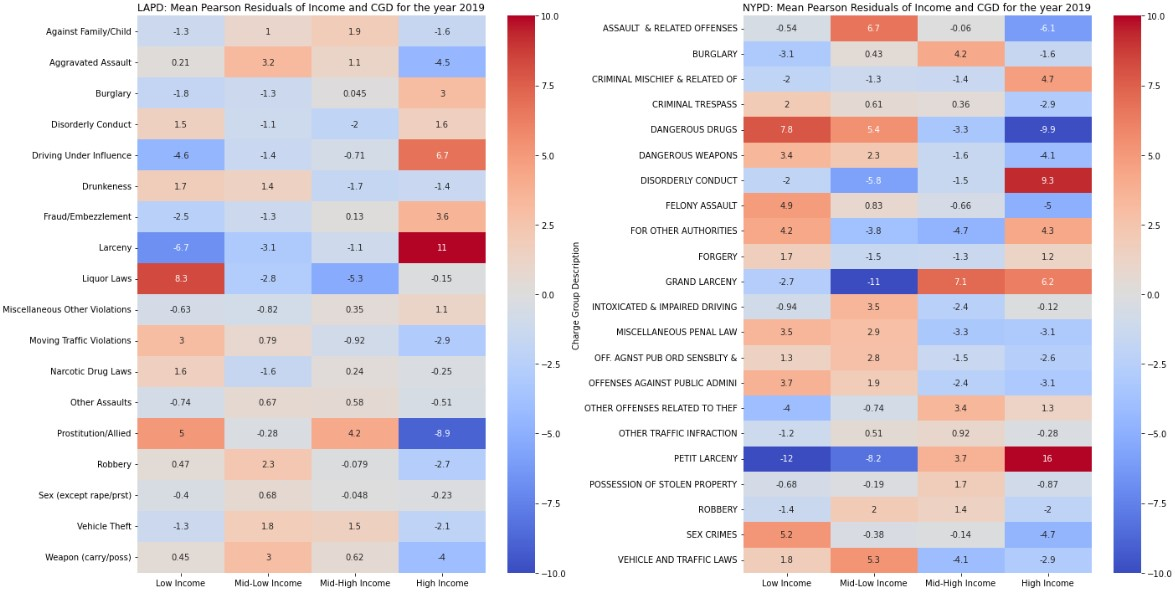
\includegraphics[scale = .7]{Graphics/LAPD_NYPD_heatmap_mean_pearson_residuals_2019.jpg}
    \caption{Mean Pearson Residuals for Income 2019 in LAPD and NYPD}
  \label{heatmap}
\end{figure}

Since our data includes the date that an arrest occurred, we can analyze changes and trends in the Pearson Residuals over time. We take the mean of 15 Pearson Residuals calculated for each year and plot the value for each charge group description from 2010 to 2019. Figure \ref{lapd_over_time} and figure \ref{nypd_over_time} visualize the mean Pearson Residuals over time for High income areas in Los Angeles and  New York City. Notice that this plot only visualizes the trends for the High-Income areas and not all income areas like in figure \ref{heatmap}.

In High iIncome areas for LAPD, shown in figure \ref{lapd_over_time}, the Mean Pearson Residuals demonstrate that over time Driving Under Influence, Larceny, and Prostitution/Allied have been high contributors to dependency. The first two charges, Driving Under Influence and Larceny, have consistently occurred more frequently than expected in High Income areas, and Prostitution/Allied occurred less frequently than expected. These plots do not provide a casual explanation as to why certain charges occur more frequently than expected in High Income Areas.

\newpage
\newgeometry{left=3cm,bottom=0.1cm}
\begin{figure}[!ht]
    \centering
    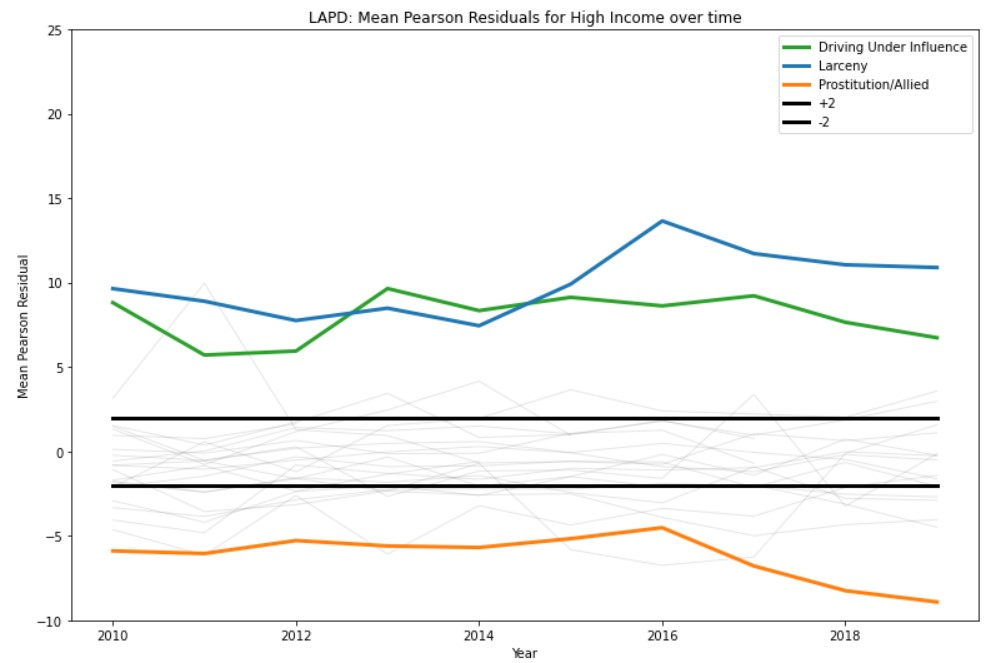
\includegraphics[scale = .7]{Graphics/LAPD_mean_pearson_residuals_over_time.jpg}
    \caption{Mean Pearson Residuals for Income Over Time in LAPD }
  \label{lapd_over_time}
\end{figure}




\begin{figure}[!ht]
    \centering
    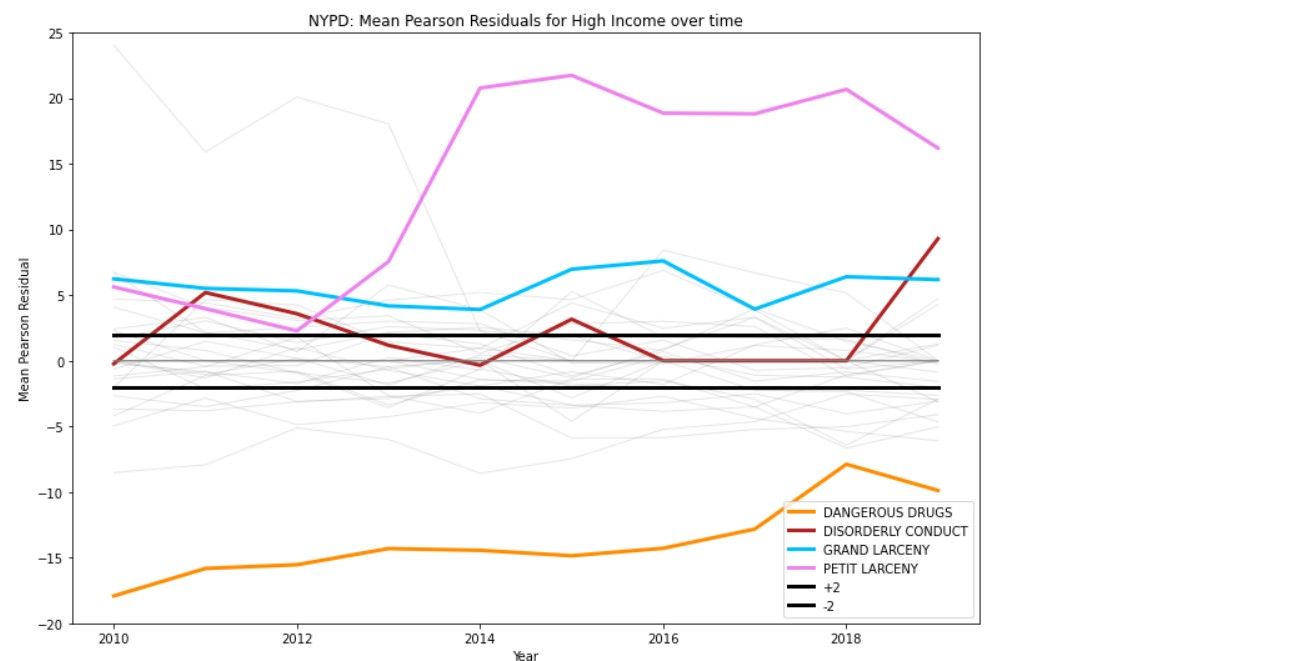
\includegraphics[scale = .7]{Graphics/NYPD_mean_pearson_residuals_over_time.jpg}
    \caption{Mean Pearson Residuals for Income Over Time in NYPD }
  \label{nypd_over_time}
\end{figure}

\newpage
\restoregeometry
 The NYPD mean Pearson Residuals for arrests in High Income  areas show that over time Dangerous Drugs, Disorderly Conduct, Grand Larceny, and Petit Larceny have been strong contributors to dependency. Of interest is the spike in mean Pearson Residual for Petit Larceny around 2013, and Petit Larceny continues to be a major contributor to dependency for several years afterwards. Between both LAPD and NYPD, Larceny has been a high contributor to dependency in high income areas.

High Income areas and areas with Low Poverty Rates have many similarities between them concerning which CGDs are leading to dependency. For instance, in  High Income areas in New York City for 2019 CGDs such as Disorderly Conduct and Petit Larceny are high contributors to dependency just as they are for areas with Low Poverty Rates. For High Income areas, Disorderly Conduct has a mean Pearson Residual value of 9.3 and Petit Larceny has a value of 16. For areas with Low Poverty Rates, Disorderly Conduct has a value of 7.6 and Petit Larceny has a value of 13. This similarity happens conversely for Low Income areas and areas with High Poverty Rates. Although not all values correspond between the groups, there are many that do. More similarities can be observed in the accompanying Jupyter Notebook linked located in our \href{https://github.com/MilesMena/Policing-Report}{GitHub repository}. 


For both departments we also applied these techniques to racial groups and CGD. During 2019, and in LAPD, we found that arrested individuals that were Black were arrested more than expected for Prostitution/Allied with a mean Pearson Residual of  $7.3$ and less than expected for Driving Under the Influence, with a mean Pearson Residual of $-6.8$. Hispanic/Latin/Mexican arrested individuals were arrested more than expected for Driving under the influence, 6, and more than expected for Drunkenness $3.4$. Individuals that were arrested and White were arrested more than expected for Narcotic Drug Laws, 4.9, and Larceny, 4.8. In NYPD there were fewer CGD and race combinations over and below $2$ and $-2$, although White arrested individuals arrested for Disorderly conduct stood out with a mean Pearson Residual of 5.\cite{github}








\section{Conclusions}



The results discussed in this paper are limited in generalizability and come with a variety of qualifications. Firstly, the use of the Chi Squared Test of Independence requires every cell in a contingency table to be full of at least $10$ occurrences, so we could only use police departments that had enough data to fulfill this requirement, like the NYPD and LAPD. Along the same lines, we could only analyze CGDs with enough occurrences for each social group, so our Chi Square Test of Independence only tells us that social group is dependent on the CGDs we had available in our data set. In selecting the years for analysis, we only analyzed years common to both data sets, 2010-2019.

Secondly, after applying these statistical techniques to the two data sets we are cautious of making comparisons between these police departments. These police departments and cities define their CGDs and laws differently, so Aggravated Assault in LAPD might not be the same as Assault 3 `I\&' Related Offenses in NYPD. We do not know if race is self reported, or if the arresting officer assigns the arrested individual a race. Also, the racial groups are not standardized, and a White Hispanic individual in NYPD could be consider as either White or Hispanic/Latin/Mexican in LAPD. Since income and poverty groups are calculated using percentiles, it is more appropriate to use these as a comparison between departments. That being said, there are several factors that influence arrests that these heat maps don't demonstrate. The FBI's Uniform Crime Reporting warns about making comparisons between departments and list factors that influence crime such as climate, modes of transportation and highway systems, crime reporting practices of the citizenry, and cultural factors and educational, recreational, and religious characteristics. \cite{UCR-stats-their-proper-use} Importantly, our data set does not represent all crime in a police departments jurisdiction because, for a multitude of reasons, some crimes aren't caught or reported.


These results indicate that there is a trend in the two police departments to arrest individuals for certain charges based on race and the economic status of the area in which the arrest takes place. We cannot and do not draw any conclusions as to why this is happening, and we can only identify which charges in specific are contributing to dependency in Los Angeles and in New York City.


\section{Future Work}

The techniques used in this paper are not unique to these police departments and can be employed on other  police departments' arrest data, if their data set is large enough. Because these tests do not suggest a cause for dependency, further investigation can be conducted to gain an insight into why some CGDs are affecting certain groups and areas differently. Further work can also be done to connect the test results for race and economic area. For example, in LAPD Hispanic/Latin/Mexican individuals are arrested more than expected for Driving Under the Influence, and in High Income areas, Driving Under the Influence also has more arrests than expected. Also, this research was motivated by the Stop LAPD Spying Coalition's report which identified Municipal Code 41.18 as a law that targeted different groups of people. The research we conducted shows that charges grouped by theme are associated, but not an exact code. Similar methods can be applied to determine if there are specific laws that arrest groups and areas differently. Finally, this research can be extended by continuing to quantify relationships within police data to create a higher level of police accountability.


%The fact that both Hispanic/Latin/Mexican arrested individuals and arrests in High Income areas are both being arrested higher than expected suggests some underlying connection that the statistical metrics we apply do not highlight. \miles{Is this last sentence borderline "suggesting causality?"}





\bibliographystyle{plain}
\bibliography{HSreference}
\appendix
\end{document}
